\documentclass[11pt,a4paper]{article}
\usepackage[utf8]{inputenc}
\usepackage{a4wide}
\usepackage{amsmath}
\usepackage{amsfonts}
\usepackage{amssymb}
\usepackage{graphicx}

\title{Distance and curvature}
\author{Hugues Talbot}

\begin{document}
\maketitle
	
	
	\section{Normals and curvature}
	
	There is a deep link between the evolution of the normal along a curve and the curvature.
	
	Let $C$ be a planar curve. To define the curvature at a point, we can consider
	the case of a straight line. We can admit that in this case the curvature is zero along the line. For a portion of a circle, the curvature is defined to be inversely proportional to the radius of the circle:
	
	\begin{equation}
	\kappa = \frac{1}{R}
	\end{equation}
	
		\begin{figure}
			\centering
			\includegraphics[width=0.5\textwidth]{Drawings/Osculating.pdf}
			\caption{The notion of an osculating circle (best local approximation) defines the curvature as the inverse of the radius of the circle.\label{fig:oscul}}
		\end{figure}
	
	More precisely, for any curve, we can locally approximate a sufficiently regular curve (${\cal C}^2$ is enough) at a point by a circle that best approximates it locally (see Fig.~\ref{fig:oscul}. This circle is tangent to $C$ and is called an {\em osculating circle}. The radius of this circle defines the curvature.
	

	
	Another way to define the curvature is to consider a point moving at a constant speed along the curve $C$. The variation of the tangent vector along the curve defines the curvature. This is equivalent to specifying the acceleration of the point.
	
	
	\begin{equation}
	\kappa = \frac{d \mathbf{T}}{ds},
	\end{equation}
	
	where $s$ is a parametrisation of the curve. Both definition of the curvature
	are in fact equivalent (see Fig.~\ref{fig:theta}). 
	
	\begin{figure}
		\centering
		\includegraphics[width=0.3\textwidth]{Drawings/theta.pdf}
		\caption{We can write $\sin d\theta \approx d\theta = \frac{ds}{R}$. As ds tends to zero, we have $R = \frac{d\theta}{ds} = \frac{d \mathbf{T}}{ds}$.\label{fig:theta}}
	\end{figure}
	
	
	\section*{Parametrisation}
	
	Let $\gamma(t)$ be a parametrisation of the curve $C$, i.e.
	
	\begin{equation}
	\gamma(t) = (x(t),y(t))
	\end{equation}
	
	This defines the position of a point on the curve over time. We assume an injective parametrisation, i.e. such that
	the speed $\gamma'(t)$ is never zero. This means 
	
	\begin{equation}
	\forall t, \|\gamma'(t)\|^2 = x'(t)^2 + y'(t)^2 > 0 
	\end{equation}
	
	In this case, we can re-paramametrise the curve with curvilinear abcissa $s$ in such a way that the speed is constant and equal to one.
	
	\begin{equation}
	\forall s, \gamma'(s)^2 = x'(s)^2 + y'(s)^2 = 1
	\end{equation} 
	
	In this parametrisation, $\gamma'$ is the unit tangent velocity vector $\mathbf{T}$. If $\mathbf{N}$ is the unit normal vector to the curve, we have
	
	\begin{equation}
	\mathbf{T}'(s) = \kappa(s)\mathbf{N}(s)
	\end{equation}
	
	We note that instead of deriving the unit tangent vector, we can also consider deriving the unit normal vector. This is because $\mathbf{N}$ is $\mathbf{T}$ rotated by $\frac{\pi}{2}$, i.e. $\mathbf{N}(x,y) = (-y'(s),x'(s))$. This yields
	
	\begin{equation}
	\mathbf{N}'(s) = \kappa(s)\mathbf{T}(s)
	\end{equation}
	
	We will make use of that fact in the next section.
	
	\section*{Level sets}
	
	In imaging it can be difficult to represent a parametric curve because of discretization effects. It is common to
	represent it by a {\em level set} (see Fig.~\ref{fig:level_set}).
	
	\begin{figure}
		\centering
		\includegraphics[width=0.5\textwidth]{Images/Level_set_method.jpg}
		\caption{Representing a curve by a level set.\label{fig:level_set}}
	\end{figure}
	
	Let $\phi(x,y)$ be a ${\cal C}^2$ function in a domain $\Omega$. We define the curve $\Gamma$ as the zero-level-set of this function
	
	\begin{equation}
	\Gamma = \{(x,y), \phi(x,y) = 0\}
	\end{equation}
	
	$\Gamma$ is a set and no longer a parametrized curve, however we can manipulate it by working on the underlying $\phi$ function. This is the main idea behind the level-set method~\cite{Sethian-level-sets-1999}.
	

	
	\section*{Level sets and curvature}
	
	Curvature is easy to define in the level set case. For any point $(x,y)$ in $\Omega$, $\nabla \phi (x,y)$ is the gradient at $(x,y)$. If we consider the level-set at $(x,y,\phi(x,y))$, i.e. the curve that passes through $(x,y)$ at level $\phi(x,y)$, 
	then $\nabla \phi(x,y)$ is the normal vector to this curve at $(x,y)$. The unit normal is given by
	
	\begin{equation}
	\mathbf{n}(x,y) = \frac{\nabla \phi}{|\nabla \phi|}(x,y)
	\end{equation}
	
	The curvature is given by the derivative of this expression. However this is a multidimensional derivative. Since $\nabla \phi$ is a vector, we must use the divergence operator:
	
	\begin{equation}
	\kappa = \nabla . \frac{\nabla \phi}{|\nabla \phi|}
	\end{equation}
	
	This is in particular true for the computation of the curvature of $\Gamma$. 
	
		\begin{figure}
			\centering
			\includegraphics[width=0.5\textwidth]{Drawings/Distance.pdf}
			\caption{The faster the normal evolves along a curve, the higher the curvature.}
		\end{figure}
		
	\section{Application to our problem}
	\subsection{First approach}
We want to calculate $n$, the number of tests along the segment necessary to compute with a reasonable tolerance to verify the segment doesn't cross a concavity of the perfusion territory:
\begin{equation}
n \propto \frac{|p_1 - p_0|}{R}
\end{equation}
$R$ is an approximation of the local curvature along the segment by estimating the divergence at each point $p_1$ and $p_2$, called $R_1$ and $R_2$ respectively :
\begin{equation}
R = max(|R_1|, |R_2|)
\end{equation} 
The figure \ref{example} illustrates the relationship between $D = |p_1 - p_0|$, $R_1$, $R_2$ and $n$. 
\begin{figure}[h!]
\centering
\includegraphics[width=0.5\textwidth]{Drawings/CurvatureTestExample.png}
\caption{When $D$ gets bigger relatively to $max(|R_1, R_2|)$, the value of $n$ is also higher to detect if the segment crosses the perfusion territory.}
\label{example}
\end{figure}

The divergence of a a continuously differentiable vector field $\omega$ is equal to the scalar value function:
\begin{equation}
div (\omega) = (\frac{\partial}{\partial x}, \frac{\partial}{\partial y}) \cdot (\omega_x, \omega_y) 
\end{equation}
\begin{equation}
div (\omega) = \left( \omega_x(x, y) - \omega_x(x-1, y) \right) + \left( \omega_y(x, y) - \omega_y(x, y - 1) \right)
\end{equation}
with
\begin{equation}
\omega_x = \nabla_x \omega = \omega (x + 1, y) - \omega (x, y)
\end{equation}
and
\begin{equation}
\omega_y = \nabla_y \omega = \omega (x, y + 1) - \omega (x, y)
\end{equation}	

\subsection{Second approach}
We are in the case of measuring the curvature along a segment, so we could use the segment information with an iterative process.
Method: the gradient vector $\Delta w(p1)$ is projected on the segment $p_1p_2$ to obtain the point $p_{proj}$. 

If $w(p_{proj}) < 0$ or  $w(p_{proj}) > 1$ then $p_{proj}$ is out of the perfusion territory, and the segment $p_1p_2$ is non valid. 

If $0 \leq w(p_{proj}) \leq 1$ then check at the half way point: $p_{semi-proj} = 0.5 * (p_1 + p_{proj}$, if $w(p_{s}) /geq \epsilon$, then we use the distance $||p_1p_{s}||$ to sample the segment $p_1p_2$, so that we define the points where to apply secant test during Kamya's procedure.

\begin{figure}[h!]
\centering
\includegraphics[width=0.35\textwidth]{Drawings/ProjectionTest.png}
\caption{The gradient of potential at $P_1$ is projected along the segment $p_1p_2$. The sampling distance is calculated as half way.}
\label{projectiontest}
\end{figure}

Note: need to make this calculation starting from $p_1$ and $p_2$, and take the sample distance out of the two. Also, the distance $p_1p_s$ might not be contained exactly k times in the segment $p_1p_2$ : how shall we adapt? 

This method is expected to be more accurate than the previous one (using divergence) because it considers the potential along the segment.


\bibliography{notes_ht.bib}
\bibliographystyle{plain}
	
\end{document}